\newpage
\section{Analysis and Design}

\subsection{Analysis}

\subsubsection{Business process modelling}

The three processes identified in Section 4.1.2 are modelled below. Diagram sources are given in a text notation for reproduction in the project's modelling tool.

Exploration process. The process begins with authentication and ends either in occupation completion and rating or in the user selecting a different occupation. The decision points are the optional orientation, the response type within a task, and the unlock evaluation on level completion.

\begin{figure}[H]
\centering
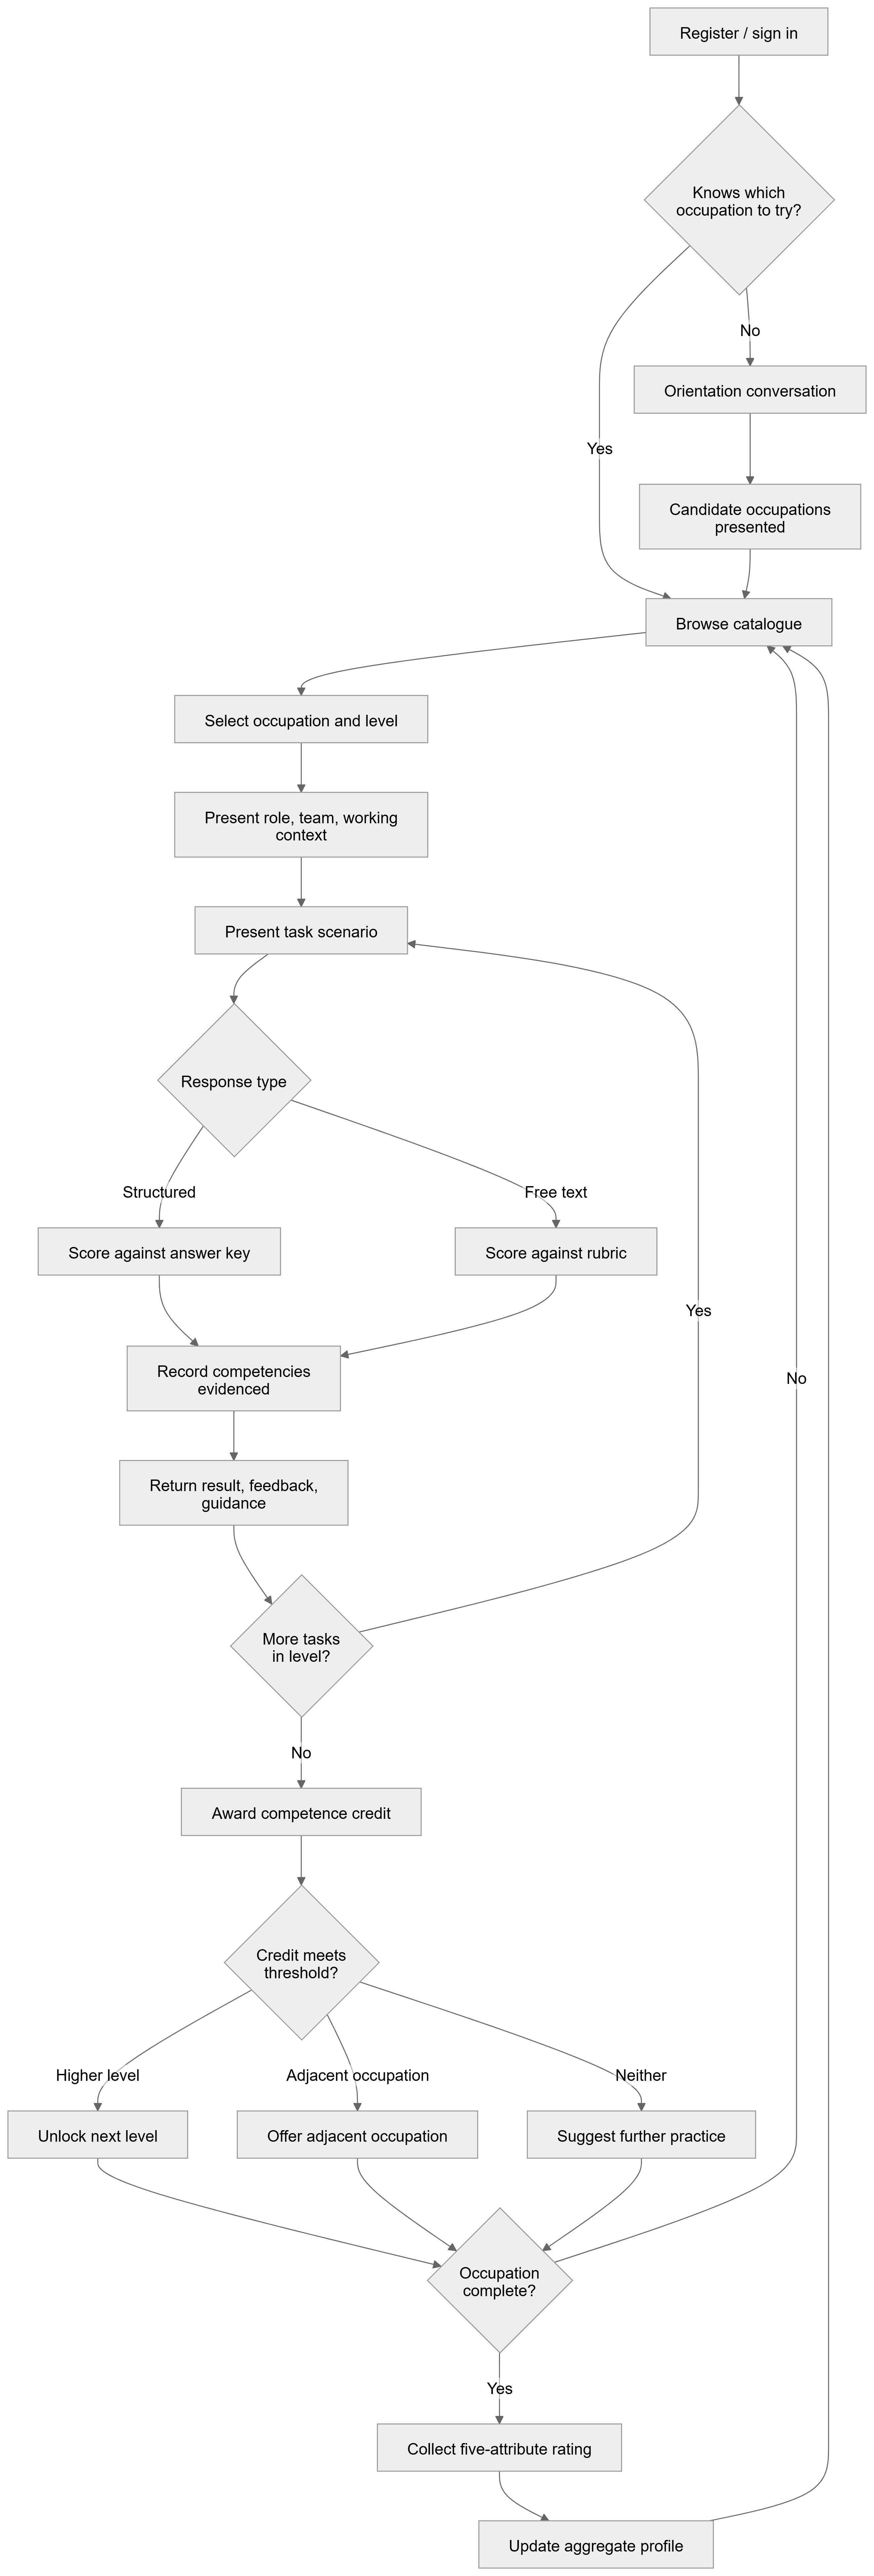
\includegraphics[width=\textwidth,height=0.9\textheight,keepaspectratio]{figures/fig1.png}
\caption{Exploration process}
\end{figure}

Content lifecycle process. This process governs occupational accuracy and is the operational expression of BR-05. Domain experts author and review content in the system; the content administrator presents, publishes, and maintains it.

\begin{figure}[H]
\centering
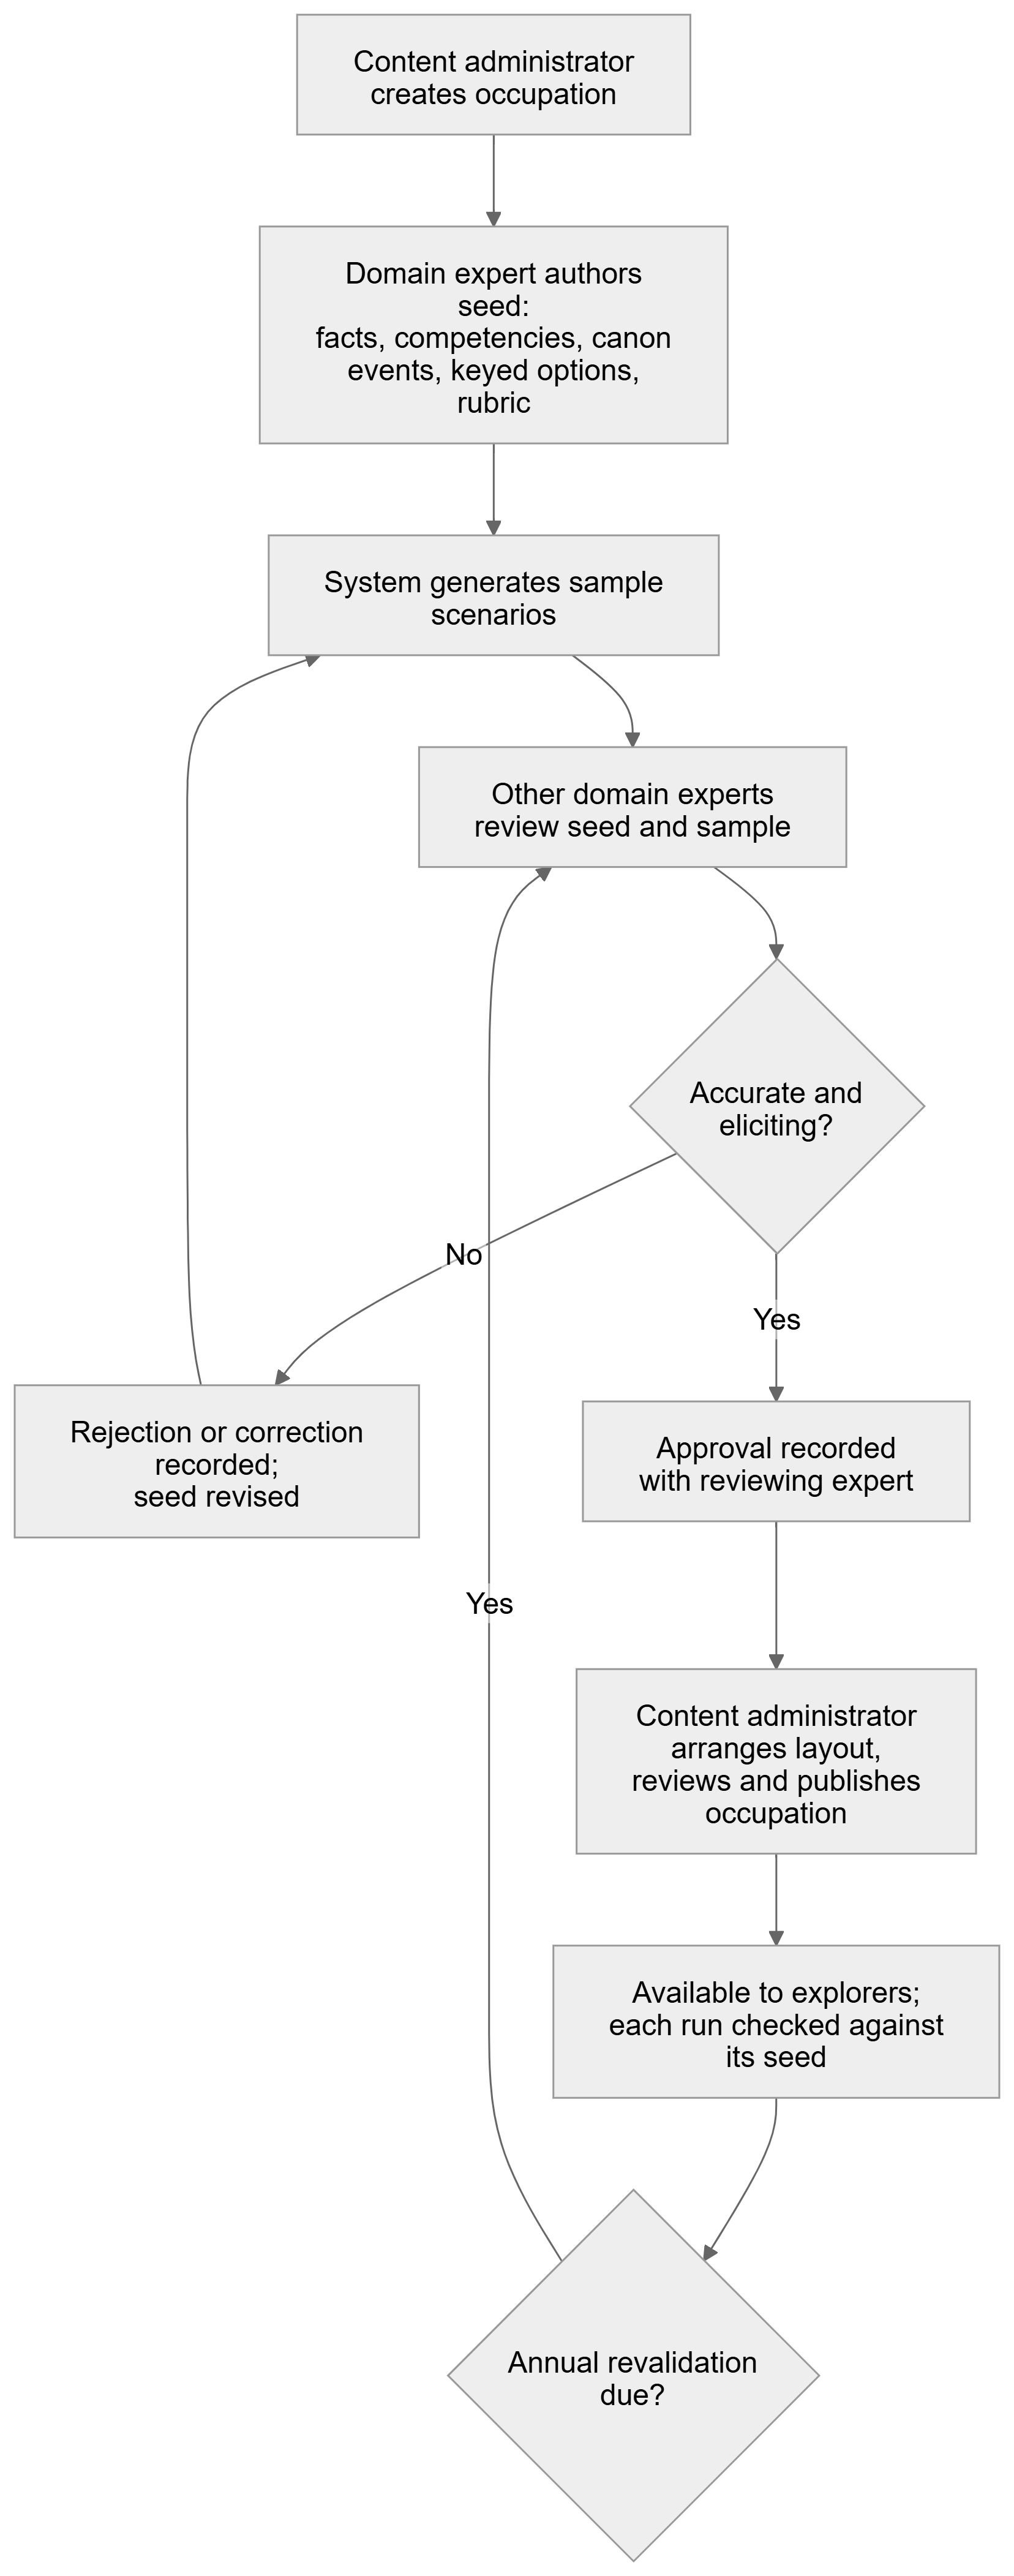
\includegraphics[width=\textwidth,height=0.9\textheight,keepaspectratio]{figures/fig2.png}
\caption{Content lifecycle process}
\end{figure}

Evaluation process. This process is internal to the project and supports RP-1 and RP-2. Experts construct reference items stratified by difficulty; generation output and assessor output are compared against them; agreement is computed with chance correction and reported per stratum, together with test--retest consistency.

\subsubsection{Use case modelling}

Four actors correspond to the user groups in Section 4.2.1. Two external systems also participate, though they are not drawn in the diagram: the model provider, which performs generation and assessment, and the occupational data source, which supplies reference data. Use cases in the diagram are named; the descriptions below also give each an identifier by actor (UC-E for the explorer, UC-D for the domain expert, UC-C for the content administrator, and UC-S for the system administrator), and the traceability matrix refers to them by name. A use case joined to another by an include relation is always performed as part of it; one joined by an extend relation is performed only under the condition stated in the flow of the use case it extends.

\begin{figure}[H]
\centering
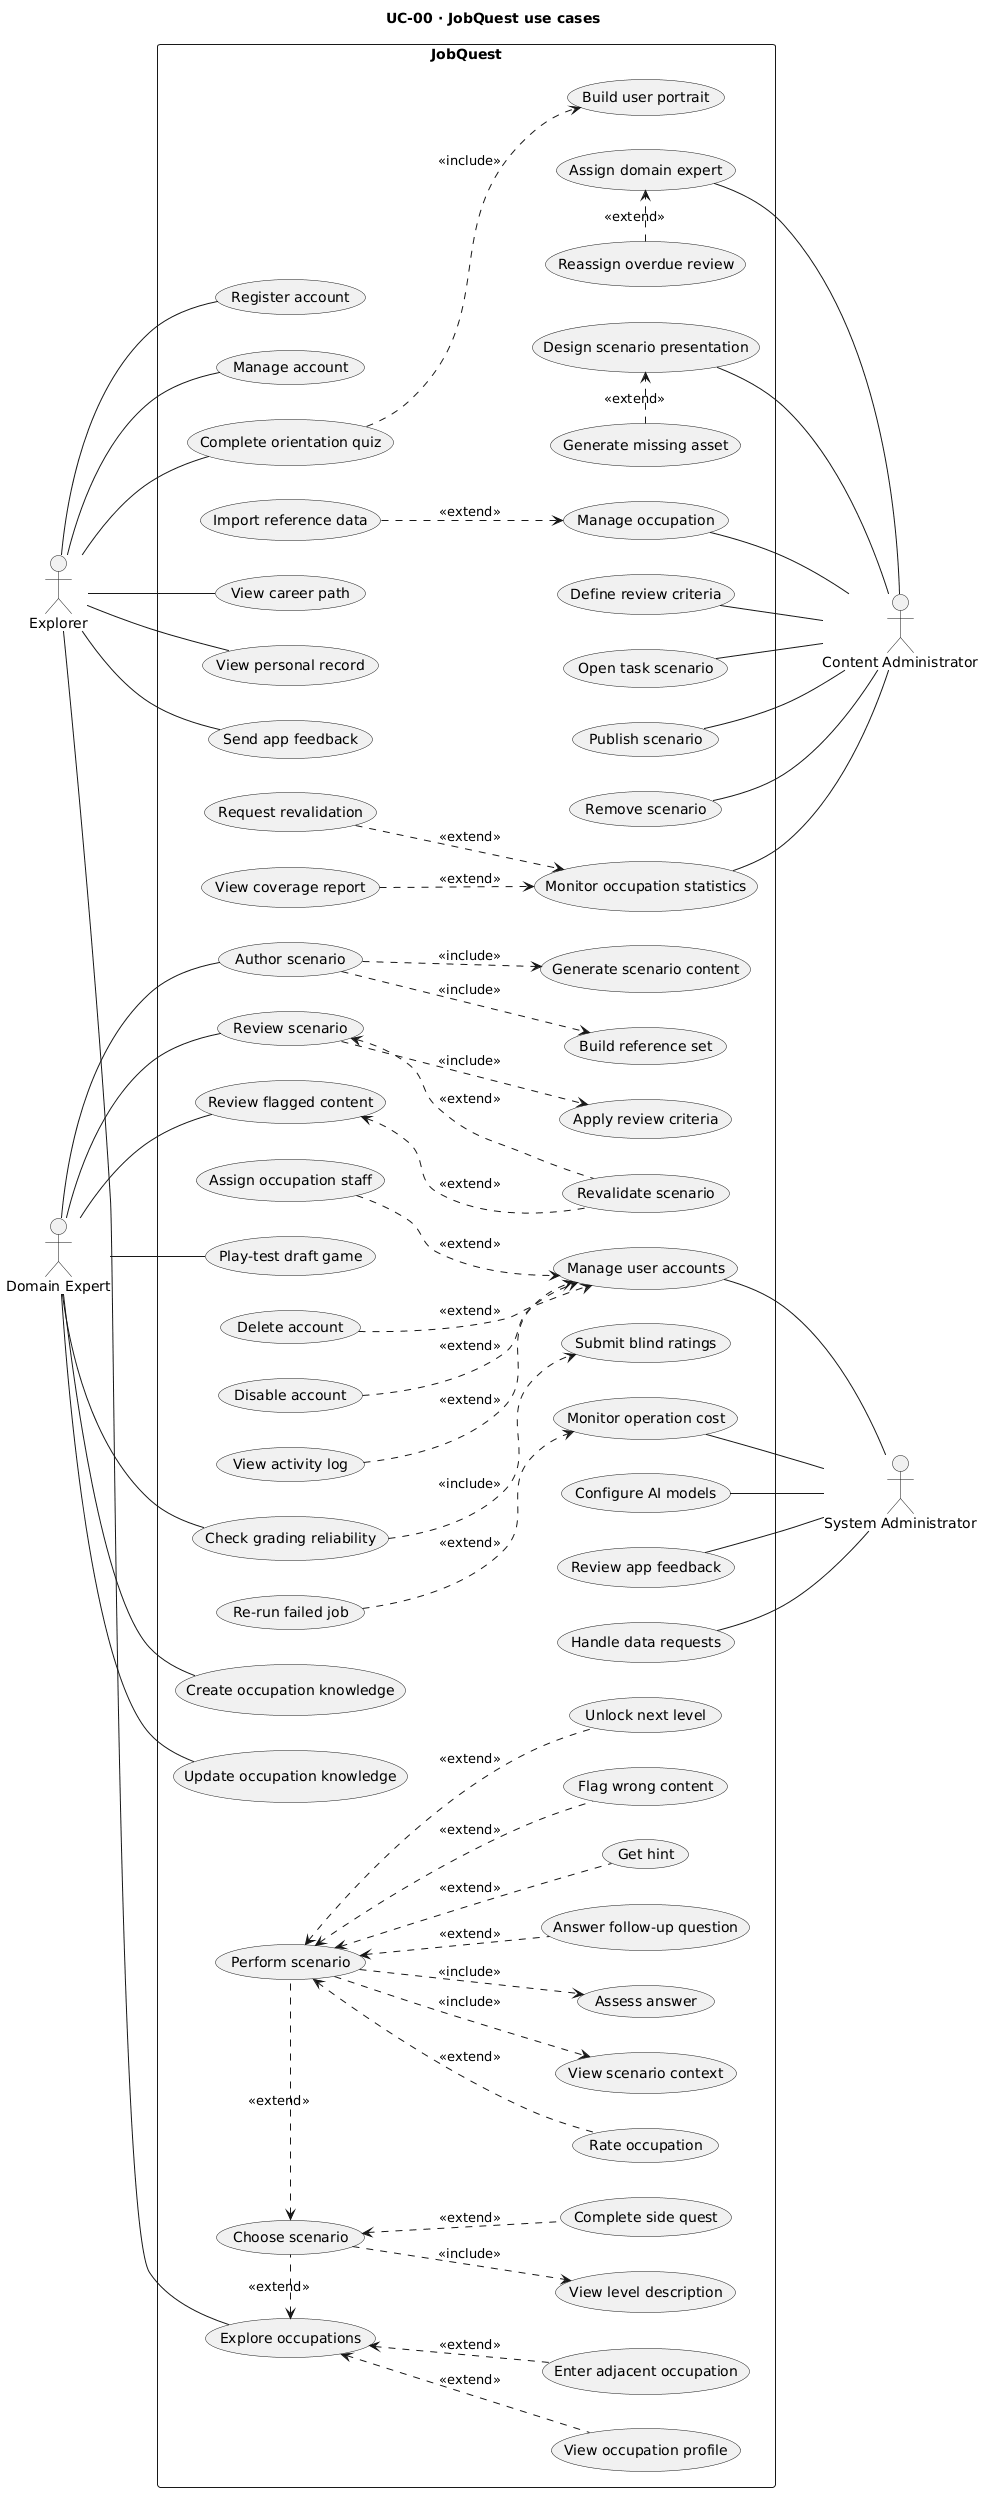
\includegraphics[width=\textwidth,height=0.9\textheight,keepaspectratio]{figures/jobquest_ucdiagram-1.png}
\caption{Use case diagram for the proposed system}
\end{figure}

Use case descriptions follow, grouped by actor. Use cases associated directly with an actor, and those involving the AI model, are described in full; small included or extending use cases are described in abbreviated form. Author scenario and Review scenario are the use cases on which RP-1 depends, and Perform scenario, through Assess answer, is the one on which RP-2 depends.

Explorer use cases.

\begin{usecase}{UC-E01}{Register account}
\ucrow{Dependencies}{%
  \ucitem{FR-01 \textit{Register, sign in, and recover the account}}
  \ucitem{NFR-05 \textit{Minimal, encrypted, deletable personal data}}
  \ucitem{NFR-17 \textit{Passwords hashed, traffic encrypted}}
  \ucitem{DR-16 \textit{User accounts, roles, assignments, and activity log}}}
\ucrow{Description}{The system shall behave as described in the following use case when \textit{a visitor without an account creates one to start exploring}.}
\ucrow{Precondition}{\textit{The visitor has opened JobQuest and is not signed in.}}
\ucsteps{Ordinary Sequence}
\ucstep{1}{Actor \textit{visitor opens JobQuest}.}
\ucstep{2}{The system \textit{checks access and shows the sign-in screen}.}
\ucstep{3}{Actor \textit{visitor chooses to register and provides the account details}.}
\ucstep{4}{The system \textit{creates the account}.}
\ucstep{5}{The system \textit{starts a session}.}
\ucstep{6}{The system \textit{opens the orientation quiz}.}
\ucrow{Postcondition}{\textit{The account exists and the explorer is signed in.}}
\ucsteps{Exceptions}
\ucstep{2}{If \textit{the visitor is already signed in}, the session continues, then this use case \textit{is cancelled}.}
\ucstep{3}{If \textit{the visitor already has an account}, the visitor \textit{signs in instead}, then this use case \textit{is cancelled}.}
\ucrow{Comments}{\textit{Only minimal personal data is collected and stored encrypted (NFR-05). Passwords are stored as salted hashes (NFR-17).}}
\end{usecase}

\begin{usecase}{UC-E02}{Manage account}
\ucrow{Dependencies}{%
  \ucitem{FR-02 \textit{Edit, sign out of, and delete the account}}
  \ucitem{FR-03 \textit{Retakable orientation quiz}}
  \ucitem{NFR-05 \textit{Minimal, encrypted, deletable personal data}}
  \ucitem{DR-16 \textit{User accounts, roles, assignments, and activity log}}}
\ucrow{Description}{The system shall behave as described in the following use case when \textit{an explorer edits, signs out of, or deletes their account, or retakes the orientation quiz}.}
\ucrow{Precondition}{\textit{The explorer is signed in.}}
\ucsteps{Ordinary Sequence}
\ucstep{1}{Actor \textit{explorer opens the profile}.}
\ucstep{2}{Actor \textit{explorer opens the account settings}.}
\ucstep{3}{Actor \textit{explorer edits the account details}.}
\ucstep{4}{The system \textit{saves the changes}.}
\ucrow{Postcondition}{\textit{The account details are up to date.}}
\ucsteps{Exceptions}
\ucstep{2}{If \textit{the explorer chooses to retake the quiz}, UC-E03 \textit{Complete orientation quiz} starts. If \textit{the explorer chooses neither}, the system \textit{opens the Galaxy Map}.}
\ucstep{3}{If \textit{the explorer signs out}, the system \textit{ends the session}.}
\ucstep{3}{If \textit{the explorer deletes the account}, the system \textit{deletes the personal data and ends the session}.}
\ucrow{Comments}{\textit{Account deletion removes personal data as defined in NFR-05.}}
\end{usecase}

\begin{usecase}{UC-E03}{Complete orientation quiz}
\ucrow{Dependencies}{%
  \ucitem{FR-03 \textit{Optional, retakable RIASEC orientation quiz}}
  \ucitem{NFR-05 \textit{Only de-identified data sent to AI providers}}
  \ucitem{DR-12 \textit{Quiz answers, RIASEC profile, and AI portrait}}
  \ucitem{Includes UC-E04 \textit{Build user portrait}}}
\ucrow{Description}{The system shall behave as described in the following use case when \textit{an explorer takes the optional RIASEC quiz to receive occupation suggestions}.}
\ucrow{Precondition}{\textit{The explorer is signed in.}}
\ucsteps{Ordinary Sequence}
\ucstep{1}{Actor \textit{explorer opens the orientation quiz and chooses to take it now}.}
\ucstep{2}{The system \textit{shows the quiz questions}.}
\ucstep{3}{Actor \textit{explorer answers every question and submits the answers}.}
\ucstep{4}{The system \textit{calculates the RIASEC profile}.}
\ucstep{5}{The system \textit{matches the profile with the O*NET interest code of each occupation and picks the five closest occupations}.}
\ucstep{6}{The system \textit{builds the user portrait} (UC-E04).}
\ucstep{7}{The system \textit{saves the profile, replacing any earlier result}.}
\ucstep{8}{Actor \textit{explorer views the description, the social index, and the five suggested occupations}.}
\ucstep{9}{Actor \textit{explorer picks an occupation}, and the system \textit{opens it}.}
\ucrow{Postcondition}{\textit{The RIASEC profile, the portrait, and the suggestions are stored.}}
\ucsteps{Exceptions}
\ucstep{1}{If \textit{the explorer skips the quiz}, the system \textit{opens the Galaxy Map}, then this use case \textit{is cancelled}.}
\ucstep{3}{If \textit{some answers are missing}, the system \textit{highlights them}, then step 3 \textit{repeats}.}
\ucstep{9}{If \textit{the explorer chooses to browse all occupations}, the system \textit{opens the Galaxy Map}.}
\ucrow{Comments}{\textit{The quiz follows Holland's RIASEC model \cite{r41}. The suggestions are computed without AI. The number of suggestions, five, is project-defined (FR-03).}}
\end{usecase}

\begin{usecase}{UC-E04}{Build user portrait}
\ucrow{Description}{The system shall behave as described in the following use case when \textit{a RIASEC profile has to be turned into a portrait}.}
\ucrow{Precondition}{\textit{The RIASEC profile has been calculated (UC-E03, step 4).}}
\ucsteps{Ordinary Sequence}
\ucstep{1}{The system \textit{takes the Social score as the social index}.}
\ucstep{2}{The system \textit{sends the de-identified profile to the AI model}.}
\ucstep{3}{The AI model \textit{writes the user description}.}
\ucstep{4}{The system \textit{checks the description}. If \textit{the check fails}, step 3 \textit{repeats}.}
\ucstep{5}{The system \textit{labels the portrait as self-reported and not validated}.}
\ucrow{Postcondition}{\textit{The portrait is stored with the profile.}}
\end{usecase}

\begin{usecase}{UC-E05}{Explore occupations}
\ucrow{Dependencies}{%
  \ucitem{FR-05 \textit{Galaxy Map and occupation profiles}}
  \ucitem{FR-06 \textit{Entry level open to every explorer}}
  \ucitem{DR-15 \textit{Occupation catalogue}}
  \ucitem{Extended by UC-E06, UC-E07, UC-E08}}
\ucrow{Description}{The system shall behave as described in the following use case when \textit{an explorer browses the published occupations on the Galaxy Map}.}
\ucrow{Precondition}{\textit{The explorer is signed in.}}
\ucsteps{Ordinary Sequence}
\ucstep{1}{Actor \textit{explorer opens the Galaxy Map}.}
\ucstep{2}{The system \textit{shows every published occupation}.}
\ucstep{3}{Actor \textit{explorer selects an occupation}.}
\ucstep{4}{The system \textit{opens the entry level of the occupation}.}
\ucstep{5}{The system \textit{opens the occupation map}.}
\ucstep{6}{Actor \textit{explorer reads the occupation profile} (UC-E06).}
\ucrow{Postcondition}{\textit{The explorer is on the occupation map with the entry level open.}}
\ucsteps{Exceptions}
\ucstep{3}{If \textit{an occupation has already been chosen}, for example from the quiz, the sequence \textit{continues at step 4}.}
\ucstep{4}{If \textit{the explorer's competencies overlap with this occupation}, UC-E07 \textit{Enter adjacent occupation} runs.}
\ucstep{6}{Actor \textit{explorer may skip the profile and choose a level} (UC-E08).}
\ucrow{Comments}{\textit{The entry level opens with zero credit and without any adjacency check (FR-06).}}
\end{usecase}

\begin{usecase}{UC-E06}{View occupation profile}
\ucrow{Description}{The system shall behave as described in the following use case when \textit{an explorer reads the profile of the selected occupation}.}
\ucrow{Precondition}{\textit{An occupation is selected.}}
\ucsteps{Ordinary Sequence}
\ucstep{1}{Actor \textit{explorer chooses to read the profile}.}
\ucstep{2}{The system \textit{shows all profile fields, the main downsides, and a description of every level}.}
\ucstep{3}{The system \textit{shows the average rating if enough ratings exist}.}
\ucrow{Postcondition}{\textit{The explorer returns to the occupation map.}}
\end{usecase}

\begin{usecase}{UC-E07}{Enter adjacent occupation}
\ucrow{Description}{The system shall behave as described in the following use case when \textit{the explorer's recorded competencies overlap with the selected occupation}.}
\ucrow{Precondition}{\textit{An occupation is selected, and the explorer has recorded competencies.}}
\ucsteps{Ordinary Sequence}
\ucstep{1}{The system \textit{compares the explorer's competencies with the adjacency data of the occupation}.}
\ucstep{2}{The system \textit{unlocks a higher starting level if the overlap conditions are met}.}
\ucstep{3}{The system \textit{keeps the entry level open}.}
\ucrow{Postcondition}{\textit{The explorer can start at the entry level or at the unlocked level.}}
\end{usecase}

\begin{usecase}{UC-E08}{Choose scenario}
\ucrow{Dependencies}{%
  \ucitem{FR-08 \textit{Enrol in levels, choose scenarios, unlock the next level}}
  \ucitem{FR-33 \textit{One active scenario per task}}
  \ucitem{DR-06 \textit{User progress}}
  \ucitem{Includes UC-E09; extended by UC-E10; extends UC-E05}}
\ucrow{Description}{The system shall behave as described in the following use case when \textit{an explorer chooses a level, enrols in it, and picks a quest}.}
\ucrow{Precondition}{\textit{The explorer is on the occupation map.}}
\ucsteps{Ordinary Sequence}
\ucstep{1}{Actor \textit{explorer chooses a level}.}
\ucstep{2}{The system \textit{shows the level description} (UC-E09).}
\ucstep{3}{The system \textit{confirms that the level is unlocked}.}
\ucstep{4}{Actor \textit{explorer enrols in the level}.}
\ucstep{5}{The system \textit{saves the enrolment}.}
\ucstep{6}{The system \textit{opens the Island Map}.}
\ucstep{7}{Actor \textit{explorer chooses a main quest}, then UC-E11 \textit{Perform scenario} starts.}
\ucrow{Postcondition}{\textit{The explorer is enrolled in the level and has chosen a scenario.}}
\ucsteps{Exceptions}
\ucstep{3}{If \textit{the level is locked}, the system \textit{shows the required credit}, then step 1 \textit{repeats}.}
\ucstep{4}{If \textit{the explorer is already enrolled}, the sequence \textit{continues at step 6}.}
\ucstep{7}{If \textit{the explorer chooses a side quest}, UC-E10 \textit{Complete side quest} runs.}
\ucrow{Comments}{\textit{A task has at most one active scenario (FR-33), so choosing a quest means choosing a task.}}
\end{usecase}

\begin{usecase}{UC-E09}{View level description}
\ucrow{Description}{The system shall behave as described in the following use case when \textit{an explorer chooses a level}.}
\ucrow{Precondition}{\textit{The explorer is on the occupation map.}}
\ucsteps{Ordinary Sequence}
\ucstep{1}{The system \textit{shows what the level involves and the credit needed to unlock it}.}
\ucrow{Postcondition}{\textit{The explorer knows what the level involves.}}
\end{usecase}

\begin{usecase}{UC-E10}{Complete side quest}
\ucrow{Description}{The system shall behave as described in the following use case when \textit{an explorer answers a side quest on the Island Map}.}
\ucrow{Precondition}{\textit{The explorer is enrolled in the level and is on the Island Map.}}
\ucsteps{Ordinary Sequence}
\ucstep{1}{Actor \textit{explorer chooses a side quest}.}
\ucstep{2}{Actor \textit{explorer answers the quick question}.}
\ucstep{3}{The system \textit{adds bonus points, recorded separately from competence credit}.}
\ucrow{Postcondition}{\textit{The bonus points are recorded.}}
\end{usecase}

\begin{usecase}{UC-E11}{Perform scenario}
\ucrow{Dependencies}{%
  \ucitem{FR-09 \textit{Show role, team, and context before each scenario}}
  \ucitem{FR-10, FR-11 \textit{Answer forms and anchored scoring}}
  \ucitem{FR-13, FR-14, FR-15 \textit{Hints, feedback, and recorded competencies}}
  \ucitem{NFR-03, NFR-04 \textit{Progress survives interruption and provider failure}}
  \ucitem{NFR-05, NFR-07 \textit{De-identified data; AI disclosure}}
  \ucitem{DR-06, DR-07 \textit{User progress; assessment records}}
  \ucitem{Includes UC-E12, UC-E13; extended by UC-E14, UC-E15, UC-E16, UC-E17, UC-E18; extends UC-E08}}
\ucrow{Description}{The system shall behave as described in the following use case when \textit{an explorer plays a published scenario of a level they are enrolled in}.}
\ucrow{Precondition}{\textit{The explorer is signed in, is enrolled in the level, and has chosen a main quest (UC-E08).}}
\ucsteps{Ordinary Sequence}
\ucstep{1}{The system \textit{loads the scenario at the saved position and shows the role, team, and goal} (UC-E12).}
\ucstep{2}{Actor \textit{explorer reads the scenario context}.}
\ucstep{3}{The system \textit{opens the activity and shows the NPC line}.}
\ucstep{4}{Actor \textit{explorer submits an answer}.}
\ucstep{5}{The system \textit{assesses the answer} (UC-E13).}
\ucstep{6}{The system \textit{shows the NPC closing line, records the competencies, and saves progress}.}
\ucstep{7}{Steps 3--6 \textit{repeat for each remaining activity}.}
\ucstep{8}{The system \textit{counts the +2 and $-1$ marks and picks the ending that matches the score}.}
\ucstep{9}{The AI model \textit{writes the strengths, the improvements, and one tip for next time}.}
\ucstep{10}{The system \textit{updates the progress bars, saves the play history and badges, and checks the credit for the next level} (UC-E17).}
\ucstep{11}{Actor \textit{explorer views the ending, the feedback, and the guidance, then returns to the Island Map}.}
\ucrow{Postcondition}{\textit{The evidence, progress, and play history are stored, and the explorer has received the ending, feedback, and guidance.}}
\ucsteps{Exceptions}
\ucstep{1}{If \textit{the scenario is not available}, the system \textit{returns the explorer to the Galaxy Map}, then this use case \textit{is cancelled}.}
\ucstep{3}{If \textit{a random event is triggered}, the system \textit{shows it}, actor \textit{explorer responds}, and the AI model \textit{grades the response as bonus soft-skill evidence}. The sequence \textit{continues at step 4}.}
\ucstep{4}{Actor \textit{explorer may open a hint} (UC-E15). The +2 mark of the activity \textit{is then lowered to 0}.}
\ucstep{4}{If \textit{the explorer leaves the scenario}, the system \textit{saves progress and returns to the Island Map}. The scenario \textit{later resumes at the saved position}.}
\ucstep{5}{If \textit{a free-text answer needs a follow-up and the limit has not been reached}, UC-E14 \textit{Answer follow-up question} runs.}
\ucstep{10}{If \textit{the credit is not enough}, the system \textit{suggests tasks to practise}.}
\ucstep{11}{If \textit{the occupation is completed}, actor \textit{explorer may rate it} (UC-E18) \textit{or open the profile}.}
\ucrow{Comments}{\textit{AI-written follow-ups and feedback must pass the output check, otherwise the expert's default is shown (FR-12, FR-14). Credit is capped per skill per scenario, so replaying never inflates it (FR-15). Random-event answers add bonus soft-skill evidence only and never lower the main score (FR-15, FR-22).}}
\end{usecase}

\begin{usecase}{UC-E12}{View scenario context}
\ucrow{Description}{The system shall behave as described in the following use case when \textit{a scenario starts}.}
\ucrow{Precondition}{\textit{The explorer has chosen a main quest.}}
\ucsteps{Ordinary Sequence}
\ucstep{1}{The system \textit{loads the scenario at the saved position}.}
\ucstep{2}{The system \textit{shows the role, the team, the goal, and the working context}.}
\ucstep{3}{Actor \textit{explorer reads the context}.}
\ucrow{Postcondition}{\textit{The context has been shown before the first activity.}}
\end{usecase}

\begin{usecase}{UC-E13}{Assess answer}
\ucrow{Dependencies}{%
  \ucitem{FR-10 \textit{Choice, ordering, prioritising, and free-text answers}}
  \ucitem{FR-11 \textit{Anchored scoring backed by quotations}}
  \ucitem{FR-13, FR-15 \textit{Hint penalty; capped competencies}}
  \ucitem{NFR-02, NFR-04, NFR-05, NFR-14, NFR-17}
  \ucitem{DR-07 \textit{Assessment records}}
  \ucitem{Included by UC-E11 and UC-E14}}
\ucrow{Description}{The system shall behave as described in the following use case when \textit{an answer submitted by the explorer has to be scored}.}
\ucrow{Precondition}{\textit{The explorer has submitted an answer to an activity.}}
\ucsteps{Ordinary Sequence}
\ucstep{1}{The system \textit{checks the answer type}.}
\ucstep{2}{The system \textit{de-identifies the free-text answer}.}
\ucstep{3}{The system \textit{sends the answer to the AI model as separated data, together with the rubric anchors}.}
\ucstep{4}{The AI model \textit{grades the answer against the anchors, quoting the explorer's words}.}
\ucstep{5}{The system \textit{checks that every quotation appears verbatim in the answer and that the score is a rubric anchor}.}
\ucstep{6}{The system \textit{keeps the evidence with the exact quotations}.}
\ucstep{7}{The system \textit{records the competencies, capped per skill per scenario}.}
\ucrow{Postcondition}{\textit{The evidence is stored with its quotation.}}
\ucsteps{Exceptions}
\ucstep{1}{If \textit{the answer is a choice, ordering, or prioritising answer}, the system \textit{scores it with the expert's scores}, then the sequence \textit{continues at step 7}.}
\ucstep{4}{If \textit{the AI provider fails}, the system \textit{keeps the progress and notifies the explorer within 10\,s} (NFR-04).}
\ucstep{5}{If \textit{a quotation is not found or the score is outside the anchors}, the system \textit{rejects the result}.}
\ucstep{7}{If \textit{a hint was used in this activity}, the system \textit{lowers +2 to 0}.}
\ucrow{Comments}{\textit{Free-text assessment finishes within 8\,s at the 95th percentile (NFR-02). Instructions written inside an answer are ignored (NFR-17). Agreement with experts is checked under NFR-14.}}
\end{usecase}

\begin{usecase}{UC-E14}{Answer follow-up question}
\ucrow{Dependencies}{%
  \ucitem{FR-12 \textit{AI-generated follow-up questions}}
  \ucitem{NFR-01 \textit{Follow-up generation time}}
  \ucitem{NFR-15 \textit{AI content stays within expert-set limits}}
  \ucitem{Extends UC-E11; includes UC-E13}}
\ucrow{Description}{The system shall behave as described in the following use case when \textit{the AI model probes a free-text answer further}.}
\ucrow{Precondition}{\textit{A free-text answer has been assessed, a follow-up is needed, and the follow-up limit of the activity has not been reached.}}
\ucsteps{Ordinary Sequence}
\ucstep{1}{The AI model \textit{generates a follow-up question within the expert's follow-up goal}.}
\ucstep{2}{The system \textit{runs the output check}.}
\ucstep{3}{The system \textit{shows the follow-up question}.}
\ucstep{4}{Actor \textit{explorer answers the follow-up question}.}
\ucstep{5}{The system \textit{assesses the answer} (UC-E13).}
\ucstep{6}{Steps 1--5 \textit{repeat while a follow-up is needed and the limit has not been reached}.}
\ucrow{Postcondition}{\textit{The follow-up answers are stored with their evidence.}}
\ucsteps{Exceptions}
\ucstep{1}{If \textit{generation takes longer than 2\,s}, the system \textit{shows progress} (NFR-01).}
\ucstep{2}{If \textit{the output check fails}, the system \textit{shows the expert's default follow-up instead}.}
\ucrow{Comments}{\textit{Follow-ups are generated within 5\,s at the 95th percentile (NFR-01), and only for free-text answers.}}
\end{usecase}

\begin{usecase}{UC-E15}{Get hint}
\ucrow{Description}{The system shall behave as described in the following use case when \textit{an explorer opens a hint during an activity}.}
\ucrow{Precondition}{\textit{The current activity has a hint.}}
\ucsteps{Ordinary Sequence}
\ucstep{1}{Actor \textit{explorer opens the hint}.}
\ucstep{2}{The system \textit{shows the hint as an NPC line}.}
\ucstep{3}{The system \textit{records the hint use and removes the +2 mark for this activity}.}
\ucrow{Postcondition}{\textit{The hint use is recorded and shown in the summary.}}
\end{usecase}

\begin{usecase}{UC-E16}{Flag wrong content}
\ucrow{Description}{The system shall behave as described in the following use case when \textit{an explorer reports wrong content in a scenario}.}
\ucrow{Precondition}{\textit{The explorer is in a scenario or is viewing its feedback.}}
\ucsteps{Ordinary Sequence}
\ucstep{1}{Actor \textit{explorer flags the content}.}
\ucstep{2}{The system \textit{stores the flag with the assessment record}.}
\ucstep{3}{The system \textit{sends the flag to a domain expert of the occupation} (UC-D07).}
\ucrow{Postcondition}{\textit{The flag has reached a domain expert.}}
\end{usecase}

\begin{usecase}{UC-E17}{Unlock next level}
\ucrow{Description}{The system shall behave as described in the following use case when \textit{a scenario ends and the credit of the level is checked}.}
\ucrow{Precondition}{\textit{The explorer has finished a scenario.}}
\ucsteps{Ordinary Sequence}
\ucstep{1}{The system \textit{compares the credit of the level with the threshold}.}
\ucstep{2}{The system \textit{unlocks the next level if the threshold is reached}. Otherwise, it \textit{suggests tasks for the missing competencies}.}
\ucrow{Postcondition}{\textit{The next level is unlocked, or tasks to practise are suggested.}}
\end{usecase}

\begin{usecase}{UC-E18}{Rate occupation}
\ucrow{Dependencies}{%
  \ucitem{FR-19 \textit{Collect occupation ratings and feedback}}
  \ucitem{NFR-06 \textit{Suppress aggregates below a minimum population}}
  \ucitem{DR-08 \textit{Five-attribute occupation ratings}}
  \ucitem{Extends UC-E11}}
\ucrow{Description}{The system shall behave as described in the following use case when \textit{an explorer rates an occupation after completing it}.}
\ucrow{Precondition}{\textit{The explorer has completed every level of the occupation.}}
\ucsteps{Ordinary Sequence}
\ucstep{1}{Actor \textit{explorer opens the occupation rating}.}
\ucstep{2}{The system \textit{confirms that the occupation is completed}.}
\ucstep{3}{Actor \textit{explorer writes feedback and rates the occupation}.}
\ucstep{4}{The system \textit{saves the rating and updates the average}.}
\ucstep{5}{The system \textit{shows the ratings of other explorers}.}
\ucstep{6}{Actor \textit{explorer views the occupation profile}.}
\ucrow{Postcondition}{\textit{The rating is stored and the average is updated.}}
\ucsteps{Exceptions}
\ucstep{2}{If \textit{the occupation is not completed}, the system \textit{keeps the rating closed}, then this use case \textit{is cancelled}.}
\ucstep{3}{If \textit{the explorer chooses to rate later}, the system \textit{records the completion only}, then the sequence \textit{continues at step 6}.}
\ucstep{5}{If \textit{there are not enough ratings}, the system \textit{hides the average}.}
\ucrow{Comments}{\textit{The rating has five attributes, a project-defined number (DR-08). Aggregates below the response-count threshold are withheld (NFR-06), and no individual rating is exposed.}}
\end{usecase}

\begin{usecase}{UC-E19}{View career path}
\ucrow{Dependencies}{%
  \ucitem{FR-17 \textit{Show the career path of each occupation level}}
  \ucitem{DR-15 \textit{Occupation catalogue, including level descriptions and future roles}}}
\ucrow{Description}{The system shall behave as described in the following use case when \textit{an explorer views where an occupation can lead}.}
\ucrow{Precondition}{\textit{The explorer is signed in and has selected an occupation.}}
\ucsteps{Ordinary Sequence}
\ucstep{1}{Actor \textit{explorer opens the career path}.}
\ucstep{2}{The system \textit{lists every level of the occupation with its role and description, as written by the domain expert}.}
\ucstep{3}{Actor \textit{explorer reads the career path}.}
\ucrow{Postcondition}{\textit{No data is changed.}}
\ucrow{Exceptions}{\textit{None.}}
\ucrow{Comments}{\textit{The content comes only from the domain expert's occupation knowledge (FR-21).}}
\end{usecase}

\begin{usecase}{UC-E20}{View personal record}
\ucrow{Dependencies}{%
  \ucitem{FR-18 \textit{Private record of attempts, points, and awards}}
  \ucitem{DR-06 \textit{User progress}}}
\ucrow{Description}{The system shall behave as described in the following use case when \textit{an explorer reviews what they have attempted and demonstrated}.}
\ucrow{Precondition}{\textit{The explorer is signed in.}}
\ucsteps{Ordinary Sequence}
\ucstep{1}{Actor \textit{explorer opens the personal record}.}
\ucstep{2}{The system \textit{rebuilds the record from the session history: attempts, expertise points, soft-skill points, and awards}.}
\ucstep{3}{Actor \textit{explorer views the record}.}
\ucrow{Postcondition}{\textit{No data is changed.}}
\ucrow{Exceptions}{\textit{None.}}
\ucrow{Comments}{\textit{The record is never accessible to other users (FR-18).}}
\end{usecase}

\begin{usecase}{UC-E21}{Send app feedback}
\ucrow{Dependencies}{%
  \ucitem{FR-20 \textit{Send app feedback and review it}}
  \ucitem{DR-18 \textit{App feedback records}}}
\ucrow{Description}{The system shall behave as described in the following use case when \textit{an explorer sends feedback about the whole app}.}
\ucrow{Precondition}{\textit{The explorer is signed in.}}
\ucsteps{Ordinary Sequence}
\ucstep{1}{Actor \textit{explorer opens the feedback form}.}
\ucstep{2}{Actor \textit{explorer writes and sends the feedback}.}
\ucstep{3}{The system \textit{stores the feedback with the time and the app version}.}
\ucstep{4}{The system \textit{adds the feedback to the review list} (UC-S10).}
\ucrow{Postcondition}{\textit{The feedback is stored and marked as not handled.}}
\ucrow{Exceptions}{\textit{None.}}
\ucrow{Comments}{\textit{App feedback is separate from occupation ratings (FR-19).}}
\end{usecase}

Domain expert use cases.

\begin{usecase}{UC-D01}{Author scenario}
\ucrow{Dependencies}{%
  \ucitem{FR-22 \textit{Author scenario context, question types, option scores, rubric, hints, random events, and side quests}}
  \ucitem{FR-23, FR-24 \textit{AI generation; reference answers}}
  \ucitem{DR-04 \textit{Scenario content}}
  \ucitem{DR-13 \textit{Scenario lifecycle record}}
  \ucitem{Includes UC-D02, UC-D03}}
\ucrow{Description}{The system shall behave as described in the following use case when \textit{the domain expert chosen as author prepares the content of a scenario for a task}.}
\ucrow{Precondition}{\textit{The content administrator has opened the scenario for the task (UC-C04), and the domain expert is its author.}}
\ucsteps{Ordinary Sequence}
\ucstep{1}{Actor \textit{domain expert opens the empty scenario}.}
\ucstep{2}{The system \textit{offers the situation types and company types}.}
\ucstep{3}{Actor \textit{domain expert chooses a situation type and a company type}.}
\ucstep{4}{Actor \textit{domain expert writes the scenario context}.}
\ucstep{5}{The system \textit{generates the scenario content} (UC-D02).}
\ucstep{6}{Actor \textit{domain expert reads the generated activities, rubric, and endings}.}
\ucstep{7}{Actor \textit{domain expert sets the question types of each activity within the level limits and scores each option}.}
\ucstep{8}{Actor \textit{domain expert checks that every rubric anchor describes observable behaviour}.}
\ucstep{9}{Actor \textit{domain expert adds sample answers} (UC-D03).}
\ucstep{10}{Actor \textit{domain expert writes the hints, random events, and side quests}.}
\ucstep{11}{The system \textit{runs the automatic checks}.}
\ucstep{12}{Actor \textit{domain expert submits the scenario for review}.}
\ucstep{13}{The system \textit{moves the scenario to Submitted}.}
\ucrow{Postcondition}{\textit{The scenario is Submitted, and the authorship of every part is recorded.}}
\ucsteps{Exceptions}
\ucstep{6}{If \textit{a part needs changes}, actor \textit{domain expert asks the AI model to revise that part}, the AI model \textit{revises it}, and the system \textit{saves a generation record}. Step 6 \textit{repeats}.}
\ucstep{11}{If \textit{a check fails}, the system \textit{shows the failed part}, actor \textit{domain expert fixes it}, then step 11 \textit{repeats}.}
\ucrow{Comments}{\textit{Steps 7--10 can be done in any order. Every free-text activity needs a follow-up goal, a default follow-up, and default feedback (FR-22). Only domain experts assigned to the occupation can author its scenarios (FR-22).}}
\end{usecase}

\begin{usecase}{UC-D02}{Generate scenario content}
\ucrow{Dependencies}{%
  \ucitem{FR-23 \textit{Generate scenario content with AI, keeping its generation history}}
  \ucitem{FR-42 \textit{Separate generation and assessment models}}
  \ucitem{DR-05 \textit{Generated scenarios with provenance}}
  \ucitem{Included by UC-D01}}
\ucrow{Description}{The system shall behave as described in the following use case when \textit{the AI model generates scenario content from the author's context}.}
\ucrow{Precondition}{\textit{The author has chosen the situation and company type and written the scenario context.}}
\ucsteps{Ordinary Sequence}
\ucstep{1}{Actor \textit{domain expert submits the context for generation}.}
\ucstep{2}{The system \textit{sends the context, the task and skills of the level, and the generation rules of the occupation to the AI model}.}
\ucstep{3}{The AI model \textit{generates the activities, the rubric, and the endings}.}
\ucstep{4}{The system \textit{runs the automated validator on the output}.}
\ucstep{5}{The system \textit{saves a generation record with the context, model, cost, and check result}.}
\ucstep{6}{The system \textit{shows the generated content to the author}.}
\ucrow{Postcondition}{\textit{The generated content and its generation record are stored.}}
\ucsteps{Exceptions}
\ucstep{3}{If \textit{the AI provider fails}, the system \textit{lists the run as failed with its cause} (UC-S08), then this use case \textit{is cancelled}.}
\ucstep{4}{If \textit{the validator fails}, the system \textit{shows the failed checks with the content}. The scenario \textit{cannot be submitted until they pass}.}
\ucrow{Comments}{\textit{The generation model is always different from the assessment model (FR-42). Every run can be traced back to its context and model (DR-05).}}
\end{usecase}

\begin{usecase}{UC-D03}{Build reference set}
\ucrow{Description}{The system shall behave as described in the following use case when \textit{the author adds sample answers with expert scores}.}
\ucrow{Precondition}{\textit{The author is preparing the scenario content (UC-D01).}}
\ucsteps{Ordinary Sequence}
\ucstep{1}{Actor \textit{domain expert writes a sample answer for a free-text activity}.}
\ucstep{2}{Actor \textit{domain expert sets its difficulty and scores it against the rubric anchors}.}
\ucstep{3}{The system \textit{validates the item}. If \textit{validation fails}, it \textit{returns the reasons}, then step 1 \textit{repeats}.}
\ucstep{4}{The system \textit{stores the item in the reference set}.}
\ucrow{Postcondition}{\textit{The sample answers are stored with expert scores, grouped by difficulty.}}
\end{usecase}

\begin{usecase}{UC-D04}{Review scenario}
\ucrow{Dependencies}{%
  \ucitem{FR-25 \textit{Review another expert's scenario against the review criteria}}
  \ucitem{FR-32, FR-34 \textit{Review criteria; reviewer assignment}}
  \ucitem{DR-13 \textit{Scenario lifecycle record}}
  \ucitem{Includes UC-D05; extended by UC-D06}}
\ucrow{Description}{The system shall behave as described in the following use case when \textit{a domain expert reviews a scenario written by another expert of the same occupation}.}
\ucrow{Precondition}{\textit{The scenario is Submitted, the content administrator has assigned this domain expert as reviewer (UC-C05), and the reviewer is not the author.}}
\ucsteps{Ordinary Sequence}
\ucstep{1}{Actor \textit{reviewer opens the scenario from the review queue}.}
\ucstep{2}{The system \textit{shows the content, the option scores, and the review criteria}.}
\ucstep{3}{Actor \textit{reviewer applies the review criteria} (UC-D05).}
\ucstep{4}{Actor \textit{reviewer approves the scenario}.}
\ucstep{5}{The system \textit{records the decision and moves the scenario to Approved}.}
\ucstep{6}{The system \textit{notifies the content administrator}.}
\ucrow{Postcondition}{\textit{The review decision is recorded with its actor and time.}}
\ucsteps{Exceptions}
\ucstep{4}{If \textit{the reviewer requests changes}, the system \textit{sends the comments to the author and returns the scenario to Draft}.}
\ucstep{4}{If \textit{the reviewer rejects the scenario}, the system \textit{closes it and moves it to Retired}.}
\ucrow{Comments}{\textit{The reviewer is never the author, and every criterion must be answered before a decision (FR-25). A rejected scenario cannot be reopened, and unapproved scenarios are never served to explorers (FR-25).}}
\end{usecase}

\begin{usecase}{UC-D05}{Apply review criteria}
\ucrow{Description}{The system shall behave as described in the following use case when \textit{a reviewer judges a scenario against the review criteria}.}
\ucrow{Precondition}{\textit{The reviewer has opened a scenario for review, and review criteria exist for the occupation.}}
\ucsteps{Ordinary Sequence}
\ucstep{1}{The system \textit{lists the criteria of the current version}.}
\ucstep{2}{Actor \textit{reviewer answers each criterion, adding comments where needed}.}
\ucstep{3}{The system \textit{allows a decision only when every criterion is answered}.}
\ucstep{4}{The system \textit{links the review to the criteria version it used}.}
\ucrow{Postcondition}{\textit{An answer is stored for every criterion.}}
\end{usecase}

\begin{usecase}{UC-D06}{Revalidate scenario}
\ucrow{Dependencies}{%
  \ucitem{FR-27 \textit{Revalidate a published scenario on request}}
  \ucitem{NFR-16 \textit{Published content immutable}}
  \ucitem{DR-13 \textit{Scenario lifecycle record}}
  \ucitem{Extends UC-D04 and UC-D07}}
\ucrow{Description}{The system shall behave as described in the following use case when \textit{a published scenario is sent back to the review queue to check that it is still accurate}.}
\ucrow{Precondition}{\textit{A domain expert or the content administrator has requested revalidation of a published scenario.}}
\ucsteps{Ordinary Sequence}
\ucstep{1}{The system \textit{adds the scenario to the review queue}.}
\ucstep{2}{Actor \textit{domain expert opens the scenario}.}
\ucstep{3}{Actor \textit{domain expert checks that the content is still accurate}.}
\ucstep{4}{Actor \textit{domain expert confirms that it is still accurate}.}
\ucstep{5}{The system \textit{records the revalidation result}.}
\ucrow{Postcondition}{\textit{The result is recorded, and the scenario stays published.}}
\ucsteps{Exceptions}
\ucstep{4}{If \textit{the content is outdated}, the system \textit{records the result, flags the scenario for replacement, and asks the content administrator to replace it} (UC-C10).}
\ucrow{Comments}{\textit{The scenario stays published and playable during revalidation (FR-27). Published content cannot be edited, so an outdated scenario is replaced, not changed (NFR-16).}}
\end{usecase}

\begin{usecase}{UC-D07}{Review flagged content}
\ucrow{Dependencies}{%
  \ucitem{FR-14 \textit{Explorers can flag wrong content to the domain expert}}
  \ucitem{DR-07 \textit{Assessment records, including explorer flags}}
  \ucitem{Extended by UC-D06}}
\ucrow{Description}{The system shall behave as described in the following use case when \textit{a domain expert handles content that an explorer has flagged as wrong}.}
\ucrow{Precondition}{\textit{An explorer has flagged content in a scenario of the expert's occupation (UC-E16).}}
\ucsteps{Ordinary Sequence}
\ucstep{1}{The system \textit{notifies the domain expert of the new flag}.}
\ucstep{2}{Actor \textit{domain expert opens the flag}.}
\ucstep{3}{The system \textit{shows the flagged content with its assessment record}.}
\ucstep{4}{Actor \textit{domain expert judges that the content is correct}.}
\ucstep{5}{The system \textit{records the decision}.}
\ucrow{Postcondition}{\textit{The flag has been handled and its decision is recorded.}}
\ucsteps{Exceptions}
\ucstep{4}{If \textit{the content is wrong}, actor \textit{domain expert starts revalidation} (UC-D06).}
\ucrow{Comments}{\textit{Every flag reaches a domain expert of that occupation (DR-07).}}
\end{usecase}

\begin{usecase}{UC-D08}{Play-test draft game}
\ucrow{Dependencies}{%
  \ucitem{FR-26 \textit{Play-test the draft game before publication}}
  \ucitem{DR-11 \textit{Play-test session flag}}
  \ucitem{DR-13 \textit{Scenario lifecycle record}}}
\ucrow{Description}{The system shall behave as described in the following use case when \textit{the author plays the draft game before it is published}.}
\ucrow{Precondition}{\textit{The content administrator has confirmed the presentation, and the system has built the draft game (UC-C07).}}
\ucsteps{Ordinary Sequence}
\ucstep{1}{The system \textit{notifies the author that the draft game is ready}.}
\ucstep{2}{Actor \textit{author plays the draft game}.}
\ucstep{3}{The system \textit{marks the session as a play-test}.}
\ucstep{4}{Actor \textit{author reports the findings}.}
\ucstep{5}{Actor \textit{author confirms that the game has no issues}.}
\ucstep{6}{The system \textit{moves the scenario to Ready}.}
\ucrow{Postcondition}{\textit{The scenario is Ready to be published.}}
\ucsteps{Exceptions}
\ucstep{5}{If \textit{the author reports a display issue}, the system \textit{returns the scenario to the content administrator for presentation} (UC-C07).}
\ucstep{5}{If \textit{the author reports a content issue}, the system \textit{returns the scenario to Draft}, so it goes back to the author and to review.}
\ucrow{Comments}{\textit{Play-test sessions are excluded from every explorer aggregate (FR-26, DR-11).}}
\end{usecase}

\begin{usecase}{UC-D09}{Check grading reliability}
\ucrow{Dependencies}{%
  \ucitem{FR-28 \textit{Report disagreements between AI and expert grading}}
  \ucitem{NFR-14 \textit{AI grading validated against expert judgment}}
  \ucitem{DR-09 \textit{Expert reference set stratified by difficulty}}
  \ucitem{Includes UC-D10}}
\ucrow{Description}{The system shall behave as described in the following use case when \textit{a domain expert checks how closely the AI grading agrees with expert grading}.}
\ucrow{Precondition}{\textit{The occupation has a reference set (UC-D03).}}
\ucsteps{Ordinary Sequence}
\ucstep{1}{Actor \textit{domain expert opens the reference samples}.}
\ucstep{2}{Actor \textit{domain expert submits blind ratings} (UC-D10).}
\ucstep{3}{The system \textit{calculates the agreement between experts}.}
\ucstep{4}{The AI model \textit{regrades all samples}.}
\ucstep{5}{The system \textit{compares the AI scores with the expert scores and lists the disagreements}.}
\ucstep{6}{Actor \textit{domain expert inspects each disagreement}.}
\ucstep{7}{Actor \textit{domain expert decides that the rubric does not need changing}.}
\ucrow{Postcondition}{\textit{The agreement figures and the disagreement list are stored.}}
\ucsteps{Exceptions}
\ucstep{5}{If \textit{there are no disagreements}, this use case \textit{ends}.}
\ucstep{7}{If \textit{the rubric needs changing}, actor \textit{domain expert asks the content administrator to replace the scenario}.}
\ucrow{Comments}{\textit{Agreement is measured with Cohen's kappa \cite{r114} for each difficulty stratum and recomputed whenever the assessment model changes (NFR-14). The disagreement list must match a recomputation over the reference set (FR-28).}}
\end{usecase}

\begin{usecase}{UC-D10}{Submit blind ratings}
\ucrow{Description}{The system shall behave as described in the following use case when \textit{a domain expert rates explorer responses or generated scenarios independently}.}
\ucrow{Precondition}{\textit{The domain expert has opened the reference samples or a generated scenario.}}
\ucsteps{Ordinary Sequence}
\ucstep{1}{The system \textit{hides the AI scores and the ratings of other experts}.}
\ucstep{2}{Actor \textit{domain expert rates each item}.}
\ucstep{3}{The system \textit{saves the ratings under this expert}.}
\ucrow{Postcondition}{\textit{A blind-rating record exists for this expert, so inter-expert agreement can be computed.}}
\end{usecase}

\begin{usecase}{UC-D11}{Create occupation knowledge}
\ucrow{Dependencies}{%
  \ucitem{FR-21 \textit{Create and update occupation knowledge}}
  \ucitem{DR-02 \textit{Competency taxonomy with observable indicators}}
  \ucitem{DR-03 \textit{Occupational adjacency with overlap measures}}}
\ucrow{Description}{The system shall behave as described in the following use case when \textit{a domain expert writes the knowledge of a newly created occupation}.}
\ucrow{Precondition}{\textit{The content administrator has created the occupation (UC-C01), and the domain expert is assigned to it.}}
\ucsteps{Ordinary Sequence}
\ucstep{1}{Actor \textit{domain expert opens the occupation}.}
\ucstep{2}{Actor \textit{domain expert writes the levels, with the role and description of each, and the salary}.}
\ucstep{3}{Actor \textit{domain expert defines the competencies and their observable indicators}.}
\ucstep{4}{Actor \textit{domain expert writes the generation rules}.}
\ucstep{5}{The system \textit{calculates the related occupations}.}
\ucstep{6}{Actor \textit{domain expert checks the related occupations}.}
\ucstep{7}{The system \textit{shows each connection on the map}.}
\ucstep{8}{Actor \textit{domain expert saves the changes}.}
\ucrow{Postcondition}{\textit{The occupation knowledge is stored with its authorship.}}
\ucsteps{Exceptions}
\ucstep{1}{If \textit{the content administrator has not created the occupation}, the system \textit{refuses}, then this use case \textit{is cancelled}.}
\ucstep{7}{If \textit{a connection does not have enough data}, the system \textit{hides it}.}
\ucrow{Comments}{\textit{Steps 2--4 and steps 5--7 can be done in any order. Every rubric criterion must resolve to a competency (FR-21). Imported O*NET and ESCO data can be used as a starting point (UC-C02).}}
\end{usecase}

\begin{usecase}{UC-D12}{Update occupation knowledge}
\ucrow{Dependencies}{%
  \ucitem{FR-21 \textit{Create and update occupation knowledge}}
  \ucitem{NFR-16 \textit{Published content immutable}}
  \ucitem{DR-02, DR-03 \textit{Competencies; adjacency}}}
\ucrow{Description}{The system shall behave as described in the following use case when \textit{a domain expert keeps the knowledge of an occupation up to date}.}
\ucrow{Precondition}{\textit{The occupation knowledge exists (UC-D11), and the domain expert is assigned to the occupation.}}
\ucsteps{Ordinary Sequence}
\ucstep{1}{Actor \textit{domain expert opens the occupation knowledge}.}
\ucstep{2}{Actor \textit{domain expert edits the levels, salary, competencies, or generation rules}.}
\ucstep{3}{The system \textit{recalculates the related occupations}.}
\ucstep{4}{Actor \textit{domain expert checks the related occupations}.}
\ucstep{5}{The system \textit{saves the changes with their authorship}.}
\ucrow{Postcondition}{\textit{The occupation knowledge is up to date.}}
\ucsteps{Exceptions}
\ucstep{3}{If \textit{a connection does not have enough data}, the system \textit{hides it}.}
\ucrow{Comments}{\textit{Published scenarios do not change when the knowledge changes (NFR-16). An affected scenario goes through revalidation instead (UC-D06).}}
\end{usecase}

Content administrator use cases.

\begin{usecase}{UC-C01}{Manage occupation}
\ucrow{Dependencies}{%
  \ucitem{FR-30 \textit{Create and manage own occupations}}
  \ucitem{FR-40 \textit{One content administrator per occupation}}
  \ucitem{DR-15 \textit{Occupation catalogue}}
  \ucitem{Extended by UC-C02}}
\ucrow{Description}{The system shall behave as described in the following use case when \textit{a content administrator adds or edits an occupation or a domain in the catalogue}.}
\ucrow{Precondition}{\textit{The content administrator is signed in.}}
\ucsteps{Ordinary Sequence}
\ucstep{1}{Actor \textit{content administrator opens the catalogue}.}
\ucstep{2}{Actor \textit{content administrator finds an occupation}.}
\ucstep{3}{Actor \textit{content administrator creates or edits the occupation}.}
\ucstep{4}{The system \textit{saves the occupation and its status}.}
\ucrow{Postcondition}{\textit{The occupation is stored with its current status.}}
\ucsteps{Exceptions}
\ucstep{1}{If \textit{the content administrator changes a domain}, actor \textit{content administrator adds, edits, or deletes the domain}. If \textit{the domain still has occupations}, the system \textit{blocks the deletion}.}
\ucstep{3}{If \textit{the occupation belongs to another content administrator}, the system \textit{refuses the action}.}
\ucstep{3}{If \textit{the content administrator imports reference data}, UC-C02 \textit{Import reference data} runs.}
\ucrow{Comments}{\textit{Status changes follow the defined lifecycle, and publication requires a completed review (FR-30). Each occupation has exactly one content administrator (FR-40).}}
\end{usecase}

\begin{usecase}{UC-C02}{Import reference data}
\ucrow{Dependencies}{%
  \ucitem{FR-31 \textit{Import O*NET and ESCO reference data}}
  \ucitem{DR-01 \textit{Occupational reference data}}
  \ucitem{Extends UC-C01}}
\ucrow{Description}{The system shall behave as described in the following use case when \textit{a content administrator starts an occupation from O*NET and ESCO data}.}
\ucrow{Precondition}{\textit{The content administrator is managing an occupation (UC-C01).}}
\ucsteps{Ordinary Sequence}
\ucstep{1}{Actor \textit{content administrator imports the O*NET and ESCO data}.}
\ucstep{2}{The system \textit{matches each record to its source identifier}.}
\ucstep{3}{Actor \textit{content administrator adapts the data to Vietnamese practice}.}
\ucstep{4}{The system \textit{notifies the domain experts of the occupation}.}
\ucrow{Postcondition}{\textit{The imported records are stored, and the domain experts can derive the competencies (UC-D11).}}
\ucsteps{Exceptions}
\ucstep{2}{If \textit{some records are not matched}, the system \textit{lists them}, then actor \textit{content administrator fixes or skips each one}.}
\ucrow{Comments}{\textit{Every imported record resolves against a source identifier (FR-31, DR-01).}}
\end{usecase}

\begin{usecase}{UC-C03}{Define review criteria}
\ucrow{Dependencies}{%
  \ucitem{FR-32 \textit{Define the scenario review criteria}}
  \ucitem{DR-19 \textit{Scenario review criteria}}}
\ucrow{Description}{The system shall behave as described in the following use case when \textit{a content administrator sets the criteria that domain experts use to review scenarios}.}
\ucrow{Precondition}{\textit{The content administrator manages the occupation.}}
\ucsteps{Ordinary Sequence}
\ucstep{1}{Actor \textit{content administrator opens the review criteria of the occupation}.}
\ucstep{2}{Actor \textit{content administrator writes or edits the criteria}.}
\ucstep{3}{The system \textit{saves the criteria as a new version}.}
\ucstep{4}{The system \textit{makes the new version available to reviewers}.}
\ucrow{Postcondition}{\textit{A versioned set of review criteria exists for the occupation.}}
\ucrow{Exceptions}{\textit{None.}}
\ucrow{Comments}{\textit{Reviews cannot start until criteria exist for the occupation, and each review links to the criteria version it used (FR-32, DR-19).}}
\end{usecase}

\begin{usecase}{UC-C04}{Open task scenario}
\ucrow{Dependencies}{%
  \ucitem{FR-33 \textit{Open one active scenario per task}}
  \ucitem{DR-13 \textit{Scenario lifecycle record}}}
\ucrow{Description}{The system shall behave as described in the following use case when \textit{a content administrator opens a new scenario for a task}.}
\ucrow{Precondition}{\textit{The content administrator manages the occupation, and the occupation has at least one domain expert.}}
\ucsteps{Ordinary Sequence}
\ucstep{1}{Actor \textit{content administrator selects a level and a task}.}
\ucstep{2}{The system \textit{checks that the task has no active scenario}.}
\ucstep{3}{Actor \textit{content administrator chooses a domain expert of the occupation as author}.}
\ucstep{4}{The system \textit{creates an empty scenario in Draft}.}
\ucstep{5}{The system \textit{notifies the author} (UC-D01).}
\ucrow{Postcondition}{\textit{The task has one active scenario in Draft, with an author.}}
\ucsteps{Exceptions}
\ucstep{2}{If \textit{the task already has an active scenario}, the system \textit{blocks the new scenario}, then this use case \textit{is cancelled}.}
\ucrow{Comments}{\textit{Retired and rejected scenarios do not count as active (FR-33).}}
\end{usecase}

\begin{usecase}{UC-C05}{Assign domain expert}
\ucrow{Dependencies}{%
  \ucitem{FR-34 \textit{Assign a reviewer with a deadline}}
  \ucitem{FR-32 \textit{Review criteria}}
  \ucitem{DR-13 \textit{Scenario lifecycle record}}
  \ucitem{Extended by UC-C06}}
\ucrow{Description}{The system shall behave as described in the following use case when \textit{a content administrator assigns a domain expert to review a submitted scenario}.}
\ucrow{Precondition}{\textit{The scenario is Submitted, and review criteria exist for the occupation (UC-C03).}}
\ucsteps{Ordinary Sequence}
\ucstep{1}{Actor \textit{content administrator opens the submitted scenario}.}
\ucstep{2}{Actor \textit{content administrator chooses a domain expert of the occupation as reviewer}.}
\ucstep{3}{Actor \textit{content administrator sets the review deadline}.}
\ucstep{4}{The system \textit{checks that the reviewer is not the author}.}
\ucstep{5}{The system \textit{moves the scenario to In Review and shows the deadline in the review queue}.}
\ucstep{6}{The system \textit{notifies the reviewer}.}
\ucstep{7}{The system \textit{reminds the reviewer before the deadline}.}
\ucrow{Postcondition}{\textit{The scenario is In Review with an assigned reviewer and a deadline.}}
\ucsteps{Exceptions}
\ucstep{4}{If \textit{the chosen expert is the author}, the system \textit{refuses}, then step 2 \textit{repeats}.}
\ucstep{7}{If \textit{the deadline passes}, UC-C06 \textit{Reassign overdue review} runs.}
\ucrow{Comments}{\textit{Assigning the author as reviewer is always refused (FR-34).}}
\end{usecase}

\begin{usecase}{UC-C06}{Reassign overdue review}
\ucrow{Description}{The system shall behave as described in the following use case when \textit{a review passes its deadline}.}
\ucrow{Precondition}{\textit{A scenario is In Review, and its deadline has passed.}}
\ucsteps{Ordinary Sequence}
\ucstep{1}{The system \textit{notifies the content administrator}.}
\ucstep{2}{Actor \textit{content administrator chooses another domain expert who is not the author}.}
\ucstep{3}{The system \textit{moves the review to the new reviewer and notifies them}.}
\ucrow{Postcondition}{\textit{The review has a new reviewer and a new deadline.}}
\end{usecase}

\begin{usecase}{UC-C07}{Design scenario presentation}
\ucrow{Dependencies}{%
  \ucitem{FR-35 \textit{Design the scenario presentation with AI}}
  \ucitem{FR-36 \textit{Bias-checked asset library}}
  \ucitem{DR-14 \textit{Presentation data and asset library}}
  \ucitem{Extended by UC-C08}}
\ucrow{Description}{The system shall behave as described in the following use case when \textit{a content administrator turns approved content into a playable game}.}
\ucrow{Precondition}{\textit{The scenario is Approved.}}
\ucsteps{Ordinary Sequence}
\ucstep{1}{Actor \textit{content administrator asks the AI model for presentation ideas}.}
\ucstep{2}{The AI model \textit{suggests characters, scenes, and question types}.}
\ucstep{3}{Actor \textit{content administrator reviews the suggestion}.}
\ucstep{4}{Actor \textit{content administrator chooses the question types from the set allowed by the author}.}
\ucstep{5}{Actor \textit{content administrator confirms the presentation}.}
\ucstep{6}{The system \textit{builds the draft game and moves the scenario to In Playtest}.}
\ucstep{7}{The system \textit{notifies the author to play-test it} (UC-D08).}
\ucrow{Postcondition}{\textit{A draft game exists, and the scenario is In Playtest.}}
\ucsteps{Exceptions}
\ucstep{3}{If \textit{the suggestion needs changes}, actor \textit{content administrator asks the AI model to change it}, then step 2 \textit{repeats}.}
\ucstep{4}{If \textit{a question type is outside the allowed set}, the system \textit{refuses it}.}
\ucstep{5}{If \textit{an asset is missing}, UC-C08 \textit{Generate missing asset} runs.}
\ucrow{Comments}{\textit{The content text is read-only in this step, so the presentation never changes what the expert approved (FR-35).}}
\end{usecase}

\begin{usecase}{UC-C08}{Generate missing asset}
\ucrow{Description}{The system shall behave as described in the following use case when \textit{the presentation needs an asset that the library does not have}.}
\ucrow{Precondition}{\textit{The content administrator is designing a presentation (UC-C07).}}
\ucsteps{Ordinary Sequence}
\ucstep{1}{Actor \textit{content administrator asks the AI model for the asset}.}
\ucstep{2}{The AI model \textit{generates the asset}.}
\ucstep{3}{The system \textit{checks the asset for bias}. If \textit{the check fails}, the asset \textit{is not added}.}
\ucstep{4}{The system \textit{adds the asset to the library with its source and bias-check result}.}
\ucrow{Postcondition}{\textit{The asset is in the library and can be used in the presentation.}}
\end{usecase}

\begin{usecase}{UC-C09}{Publish scenario}
\ucrow{Dependencies}{%
  \ucitem{FR-37 \textit{Publish a scenario after review and play-test}}
  \ucitem{NFR-15, NFR-16 \textit{Published content matches approved content and is immutable}}
  \ucitem{DR-05, DR-13 \textit{Provenance; lifecycle record}}}
\ucrow{Description}{The system shall behave as described in the following use case when \textit{a content administrator releases a ready scenario to explorers}.}
\ucrow{Precondition}{\textit{The scenario is Ready, so it has been approved and play-tested.}}
\ucsteps{Ordinary Sequence}
\ucstep{1}{Actor \textit{content administrator opens the ready scenario}.}
\ucstep{2}{Actor \textit{content administrator sets the effective date and writes a release note}.}
\ucstep{3}{Actor \textit{content administrator publishes the scenario}.}
\ucstep{4}{The system \textit{publishes and locks the content}.}
\ucstep{5}{The system \textit{logs the status change}.}
\ucrow{Postcondition}{\textit{The scenario is Published and served to explorers from the effective date.}}
\ucsteps{Exceptions}
\ucstep{3}{If \textit{the scenario is not Ready}, the publish action \textit{is disabled}.}
\ucrow{Comments}{\textit{Published content is identical to the approved content (NFR-15), and every later write attempt is refused (NFR-16).}}
\end{usecase}

\begin{usecase}{UC-C10}{Remove scenario}
\ucrow{Dependencies}{%
  \ucitem{FR-38 \textit{Retire or delete a published scenario}}
  \ucitem{FR-33 \textit{One active scenario per task}}
  \ucitem{NFR-16 \textit{Published content immutable}}
  \ucitem{DR-13 \textit{Scenario lifecycle record}}}
\ucrow{Description}{The system shall behave as described in the following use case when \textit{a content administrator removes a published scenario, for example because it is outdated}.}
\ucrow{Precondition}{\textit{The content administrator manages the occupation, and the scenario is Published.}}
\ucsteps{Ordinary Sequence}
\ucstep{1}{Actor \textit{content administrator chooses the published scenario}.}
\ucstep{2}{Actor \textit{content administrator confirms the deletion}.}
\ucstep{3}{The system \textit{checks whether any explorer has played the scenario}.}
\ucstep{4}{The system \textit{retires the scenario and keeps its history}.}
\ucrow{Postcondition}{\textit{The scenario is no longer served, and the task has no active scenario.}}
\ucsteps{Exceptions}
\ucstep{3}{If \textit{the scenario has never been played}, the system \textit{deletes it permanently}.}
\ucstep{4}{If \textit{the content administrator wants to replace it}, actor \textit{content administrator opens a new scenario for the same task} (UC-C04).}
\ucrow{Comments}{\textit{Published content cannot be edited (NFR-16). Replacing a scenario therefore means removing the old one first, since a task has at most one active scenario (FR-33).}}
\end{usecase}

\begin{usecase}{UC-C11}{Monitor occupation statistics}
\ucrow{Dependencies}{%
  \ucitem{FR-39 \textit{Monitor own occupations: statistics and coverage}}
  \ucitem{NFR-06 \textit{Suppress aggregates below a minimum population}}
  \ucitem{DR-11 \textit{Play-test session flag}}
  \ucitem{Extended by UC-C12, UC-C13}}
\ucrow{Description}{The system shall behave as described in the following use case when \textit{a content administrator checks how the occupation's scenarios perform}.}
\ucrow{Precondition}{\textit{The content administrator manages the occupation.}}
\ucsteps{Ordinary Sequence}
\ucstep{1}{Actor \textit{content administrator opens the statistics}.}
\ucstep{2}{The system \textit{summarises the plays and scores, summarises the ratings, loads the AI grading reliability, and counts the reference samples}.}
\ucstep{3}{Actor \textit{content administrator reviews the statistics}.}
\ucrow{Postcondition}{\textit{No data is changed.}}
\ucsteps{Exceptions}
\ucstep{2}{If \textit{a group is below the minimum population}, the system \textit{withholds its figures and states why}.}
\ucstep{3}{If \textit{practice has changed}, actor \textit{content administrator requests revalidation} (UC-C13).}
\ucstep{3}{Actor \textit{content administrator may open the coverage report} (UC-C12).}
\ucrow{Comments}{\textit{Figures match stored records (FR-39), and play-test sessions are excluded (DR-11).}}
\end{usecase}

\begin{usecase}{UC-C12}{View coverage report}
\ucrow{Description}{The system shall behave as described in the following use case when \textit{a content administrator checks which tasks of the occupation have a published scenario}.}
\ucrow{Precondition}{\textit{The content administrator is viewing the statistics (UC-C11).}}
\ucsteps{Ordinary Sequence}
\ucstep{1}{Actor \textit{content administrator opens the coverage report}.}
\ucstep{2}{The system \textit{shows, for each level and task, the status of its scenario from the stored metadata}.}
\ucrow{Postcondition}{\textit{No data is changed.}}
\end{usecase}

\begin{usecase}{UC-C13}{Request revalidation}
\ucrow{Description}{The system shall behave as described in the following use case when \textit{a content administrator suspects that a published scenario is outdated}.}
\ucrow{Precondition}{\textit{The content administrator is viewing the statistics (UC-C11).}}
\ucsteps{Ordinary Sequence}
\ucstep{1}{Actor \textit{content administrator requests revalidation of a published scenario}.}
\ucstep{2}{The system \textit{sends the scenario to the review queue, keeping it published}.}
\ucstep{3}{The system \textit{notifies the domain experts of the occupation} (UC-D06).}
\ucrow{Postcondition}{\textit{The scenario is in the review queue and still playable.}}
\end{usecase}

System administrator use cases.

\begin{usecase}{UC-S01}{Manage user accounts}
\ucrow{Dependencies}{%
  \ucitem{FR-41 \textit{Manage all user accounts, roles, and role-based access}}
  \ucitem{DR-16 \textit{User accounts, roles, assignments, and activity log}}
  \ucitem{Extended by UC-S02, UC-S03, UC-S04, UC-S05}}
\ucrow{Description}{The system shall behave as described in the following use case when \textit{a system administrator manages the accounts and roles of explorers and staff}.}
\ucrow{Precondition}{\textit{The system administrator is signed in.}}
\ucsteps{Ordinary Sequence}
\ucstep{1}{Actor \textit{system administrator opens the account list}.}
\ucstep{2}{The system \textit{shows every account, explorers and staff, with its role}.}
\ucstep{3}{Actor \textit{system administrator chooses an account}.}
\ucstep{4}{Actor \textit{system administrator grants or changes the role of the account}.}
\ucstep{5}{The system \textit{saves the change and logs the action}.}
\ucrow{Postcondition}{\textit{The account has the intended role, and the action is logged.}}
\ucsteps{Exceptions}
\ucstep{4}{If \textit{the account is a staff member who needs an occupation}, UC-S02 \textit{Assign occupation staff} runs.}
\ucstep{4}{If \textit{the system administrator needs the account's history}, UC-S03 \textit{View activity log} runs.}
\ucstep{4}{If \textit{the account must be stopped}, UC-S04 \textit{Disable account} or UC-S05 \textit{Delete account} runs.}
\ucrow{Comments}{\textit{Staff sign in on the shared login screen and see only the work for their assigned occupations. Wrong-role access to admin screens is refused (FR-41).}}
\end{usecase}

\begin{usecase}{UC-S02}{Assign occupation staff}
\ucrow{Description}{The system shall behave as described in the following use case when \textit{a system administrator decides who manages an occupation}.}
\ucrow{Precondition}{\textit{The occupation exists, and the staff accounts have the right roles.}}
\ucsteps{Ordinary Sequence}
\ucstep{1}{Actor \textit{system administrator chooses an occupation}.}
\ucstep{2}{Actor \textit{system administrator assigns one content administrator and one or more domain experts}.}
\ucstep{3}{The system \textit{checks that the occupation has exactly one content administrator and at least one domain expert}.}
\ucstep{4}{The system \textit{saves the assignment}. If \textit{the occupation moves to another content administrator}, its pending work \textit{moves too}.}
\ucrow{Postcondition}{\textit{The occupation has its staff, and they can see its work.}}
\end{usecase}

\begin{usecase}{UC-S03}{View activity log}
\ucrow{Description}{The system shall behave as described in the following use case when \textit{a system administrator checks what an account has done}.}
\ucrow{Precondition}{\textit{The system administrator has chosen an account (UC-S01).}}
\ucsteps{Ordinary Sequence}
\ucstep{1}{Actor \textit{system administrator opens the activity log of the account}.}
\ucstep{2}{The system \textit{shows every logged action of the account with its time}.}
\ucrow{Postcondition}{\textit{No data is changed.}}
\end{usecase}

\begin{usecase}{UC-S04}{Disable account}
\ucrow{Description}{The system shall behave as described in the following use case when \textit{a system administrator stops an account from being used}.}
\ucrow{Precondition}{\textit{The system administrator has chosen an account (UC-S01).}}
\ucsteps{Ordinary Sequence}
\ucstep{1}{Actor \textit{system administrator disables the account}.}
\ucstep{2}{The system \textit{blocks every later sign-in of the account and logs the action}.}
\ucrow{Postcondition}{\textit{The account cannot sign in, and its data is kept.}}
\end{usecase}

\begin{usecase}{UC-S05}{Delete account}
\ucrow{Description}{The system shall behave as described in the following use case when \textit{a system administrator removes an account}.}
\ucrow{Precondition}{\textit{The system administrator has chosen an account (UC-S01).}}
\ucsteps{Ordinary Sequence}
\ucstep{1}{Actor \textit{system administrator deletes the account}.}
\ucstep{2}{The system \textit{deletes the personal data as defined in NFR-05}.}
\ucstep{3}{The system \textit{keeps the records written by staff, such as scenarios and reviews}.}
\ucrow{Postcondition}{\textit{The personal data of the account is removed.}}
\end{usecase}

\begin{usecase}{UC-S06}{Configure AI models}
\ucrow{Dependencies}{%
  \ucitem{FR-42 \textit{Configure separate generation and assessment models}}
  \ucitem{NFR-05 \textit{No training on submitted data, no retention}}
  \ucitem{NFR-12, NFR-14 \textit{Replaceable provider; grading validated against experts}}
  \ucitem{DR-17 \textit{Platform settings}}}
\ucrow{Description}{The system shall behave as described in the following use case when \textit{a system administrator chooses which models generate content and which assess answers}.}
\ucrow{Precondition}{\textit{The system administrator is signed in.}}
\ucsteps{Ordinary Sequence}
\ucstep{1}{Actor \textit{system administrator opens the model configuration}.}
\ucstep{2}{Actor \textit{system administrator chooses the provider and model for generation}.}
\ucstep{3}{Actor \textit{system administrator chooses the provider and model for assessment}.}
\ucstep{4}{The system \textit{checks that the two providers are different}.}
\ucstep{5}{The system \textit{saves the configuration as a new version with its actor and time}.}
\ucrow{Postcondition}{\textit{The new models are used from the next AI request.}}
\ucsteps{Exceptions}
\ucstep{4}{If \textit{the same provider is chosen for both roles}, the system \textit{rejects the configuration}, then step 3 \textit{repeats}.}
\ucrow{Comments}{\textit{Changing a provider needs no change to authored content (NFR-12). When the assessment model changes, expert agreement is recomputed (NFR-14). Providers are set to keep no submitted data and not to train on it (NFR-05).}}
\end{usecase}

\begin{usecase}{UC-S07}{Monitor operation cost}
\ucrow{Dependencies}{%
  \ucitem{FR-43 \textit{Monitor usage, cost, and errors}}
  \ucitem{NFR-11 \textit{Session cost within the configured ceiling}}
  \ucitem{DR-10 \textit{Operational telemetry}}
  \ucitem{Extended by UC-S08}}
\ucrow{Description}{The system shall behave as described in the following use case when \textit{a system administrator checks usage, cost, and errors}.}
\ucrow{Precondition}{\textit{The system administrator is signed in.}}
\ucsteps{Ordinary Sequence}
\ucstep{1}{Actor \textit{system administrator opens the monitoring screen}.}
\ucstep{2}{The system \textit{shows the usage, the cost per session, and the errors}.}
\ucstep{3}{Actor \textit{system administrator compares the cost with the budget}.}
\ucrow{Postcondition}{\textit{No data is changed.}}
\ucsteps{Exceptions}
\ucstep{2}{If \textit{the cost crosses the configured threshold}, the system \textit{raises an alert}.}
\ucstep{3}{If \textit{there are failed AI jobs}, UC-S08 \textit{Re-run failed job} runs.}
\ucrow{Comments}{\textit{The cost of each session must stay within the configured ceiling (NFR-11).}}
\end{usecase}

\begin{usecase}{UC-S08}{Re-run failed job}
\ucrow{Description}{The system shall behave as described in the following use case when \textit{a generation or grading run has failed}.}
\ucrow{Precondition}{\textit{The system administrator is on the monitoring screen (UC-S07).}}
\ucsteps{Ordinary Sequence}
\ucstep{1}{The system \textit{lists the failed generation and grading runs with their cause}.}
\ucstep{2}{Actor \textit{system administrator re-runs a failed job}.}
\ucstep{3}{The system \textit{runs the job again and records the result}.}
\ucrow{Postcondition}{\textit{The job has been run again, and its result is recorded.}}
\end{usecase}

\begin{usecase}{UC-S09}{Handle data requests}
\ucrow{Dependencies}{%
  \ucitem{FR-44 \textit{Handle data requests and data-protection settings}}
  \ucitem{NFR-05 \textit{Minimal, encrypted, deletable personal data}}}
\ucrow{Description}{The system shall behave as described in the following use case when \textit{a system administrator handles a data-subject request or changes the data-protection settings}.}
\ucrow{Precondition}{\textit{A data request has been received, and the system administrator is signed in.}}
\ucsteps{Ordinary Sequence}
\ucstep{1}{Actor \textit{system administrator opens the data request}.}
\ucstep{2}{Actor \textit{system administrator completes the request, for example a deletion}.}
\ucstep{3}{The system \textit{logs the completed request}.}
\ucrow{Postcondition}{\textit{The request is completed and logged.}}
\ucsteps{Exceptions}
\ucstep{2}{If \textit{the system administrator changes the data-protection settings}, the system \textit{applies them from the next computation}.}
\ucrow{Comments}{\textit{A transfer impact assessment is documented and kept current for each AI provider (FR-44).}}
\end{usecase}

\begin{usecase}{UC-S10}{Review app feedback}
\ucrow{Dependencies}{%
  \ucitem{FR-20 \textit{Send app feedback and review it}}
  \ucitem{DR-18 \textit{App feedback records}}}
\ucrow{Description}{The system shall behave as described in the following use case when \textit{a system administrator reviews feedback sent about the app}.}
\ucrow{Precondition}{\textit{The system administrator is signed in.}}
\ucsteps{Ordinary Sequence}
\ucstep{1}{Actor \textit{system administrator opens the feedback review list}.}
\ucstep{2}{The system \textit{shows each item with its text, time, app version, and status}.}
\ucstep{3}{Actor \textit{system administrator reads an item and marks it as handled}.}
\ucstep{4}{The system \textit{saves the new status}.}
\ucrow{Postcondition}{\textit{The feedback item is marked as handled.}}
\ucrow{Exceptions}{\textit{None.}}
\ucrow{Comments}{\textit{Explorers send this feedback through UC-E21.}}
\end{usecase}

The traceability matrix below traces every requirement to the use case realising it, so that no requirement is left unrealised and no use case introduces behaviour the requirements do not specify. Use cases are listed by actor, in the order explorer, domain expert, content administrator, and system administrator, each followed by the use cases it includes or is extended by.

{\small
\begin{longtable}{|>{\raggedright\arraybackslash}p{\dimexpr 0.367\textwidth-2\tabcolsep-\arrayrulewidth\relax}|>{\raggedright\arraybackslash}p{\dimexpr 0.224\textwidth-2\tabcolsep-\arrayrulewidth\relax}|>{\raggedright\arraybackslash}p{\dimexpr 0.224\textwidth-2\tabcolsep-\arrayrulewidth\relax}|>{\raggedright\arraybackslash}p{\dimexpr 0.181\textwidth-2\tabcolsep-\arrayrulewidth\relax}|}
\caption{Traceability from requirements to use cases.} \\
\hline
\textbf{Use case} & \textbf{Functional} & \textbf{Non-functional} & \textbf{Data} \\ \hline
\endfirsthead
\hline
\textbf{Use case} & \textbf{Functional} & \textbf{Non-functional} & \textbf{Data} \\ \hline
\endhead
Register account & FR-01 & NFR-05, NFR-17 & DR-16 \\ \hline
Manage account & FR-02 & NFR-05 & DR-16 \\ \hline
Complete orientation quiz & FR-03 & NFR-08 & DR-01, DR-12 \\ \hline
Build user portrait & FR-04 & NFR-05, NFR-07 & DR-12 \\ \hline
View career path & FR-17 & --- & DR-15 \\ \hline
View personal record & FR-18 & NFR-05 & DR-06, DR-07 \\ \hline
Send app feedback & FR-20 & --- & DR-18 \\ \hline
Explore occupations & FR-05, FR-06 & NFR-08, NFR-13, NFR-18, NFR-19 & DR-01, DR-15 \\ \hline
View occupation profile & FR-05 & NFR-06 & DR-08, DR-15 \\ \hline
Enter adjacent occupation & FR-07 & --- & DR-02, DR-03, DR-06 \\ \hline
Choose scenario & FR-08 & --- & DR-06 \\ \hline
View level description & FR-05 & --- & DR-15 \\ \hline
Complete side quest & FR-16 & --- & DR-04, DR-06 \\ \hline
Perform scenario & FR-10, FR-15 & NFR-03, NFR-04, NFR-07, NFR-11, NFR-13, NFR-19 & DR-04, DR-05, DR-06 \\ \hline
View scenario context & FR-09 & NFR-09 & DR-04 \\ \hline
Assess answer & FR-11, FR-14, FR-15 & NFR-02, NFR-05, NFR-07, NFR-14, NFR-15, NFR-17 & DR-07 \\ \hline
Get hint & FR-13 & --- & DR-07 \\ \hline
Answer follow-up question & FR-12 & NFR-01, NFR-15, NFR-17 & DR-07 \\ \hline
Flag wrong content & FR-14 & --- & DR-07 \\ \hline
Unlock next level & FR-08 & --- & DR-06 \\ \hline
Rate occupation & FR-19 & NFR-06 & DR-08 \\ \hline
Author scenario & FR-22 & NFR-10, NFR-16 & DR-04 \\ \hline
Generate scenario content & FR-23 & NFR-11, NFR-12 & DR-05, DR-10 \\ \hline
Build reference set & FR-24 & --- & DR-09 \\ \hline
Review scenario & FR-25 & NFR-15, NFR-16 & DR-13 \\ \hline
Apply review criteria & FR-25 & --- & DR-19 \\ \hline
Revalidate scenario & FR-27 & NFR-16 & DR-13 \\ \hline
Review flagged content & FR-14 & --- & DR-07 \\ \hline
Play-test draft game & FR-26 & --- & DR-11 \\ \hline
Check grading reliability & FR-28 & NFR-14 & DR-07, DR-09 \\ \hline
Submit blind ratings & FR-29 & --- & DR-09 \\ \hline
Create occupation knowledge & FR-21 & NFR-10 & DR-01, DR-02, DR-03, DR-15 \\ \hline
Update occupation knowledge & FR-21 & --- & DR-02, DR-03, DR-15 \\ \hline
Manage occupation & FR-30 & NFR-10, NFR-16 & DR-13, DR-15 \\ \hline
Import reference data & FR-31 & --- & DR-01 \\ \hline
Assign domain expert & FR-34 & --- & DR-13, DR-16 \\ \hline
Reassign overdue review & FR-34 & --- & DR-13 \\ \hline
Design scenario presentation & FR-35 & NFR-15 & DR-14 \\ \hline
Generate missing asset & FR-36 & --- & DR-14 \\ \hline
Define review criteria & FR-32 & --- & DR-19 \\ \hline
Open task scenario & FR-33 & --- & DR-13 \\ \hline
Publish scenario & FR-37 & NFR-15, NFR-16 & DR-13 \\ \hline
Remove scenario & FR-38 & NFR-16 & DR-13 \\ \hline
Monitor occupation statistics & FR-39 & NFR-06 & DR-06, DR-08, DR-11 \\ \hline
Request revalidation & FR-27 & --- & DR-13 \\ \hline
View coverage report & FR-39 & --- & DR-04, DR-15 \\ \hline
Manage user accounts & FR-41 & NFR-17 & DR-16 \\ \hline
Assign occupation staff & FR-40 & --- & DR-16 \\ \hline
Disable account & FR-41 & --- & DR-16 \\ \hline
Delete account & FR-41 & NFR-05 & DR-16 \\ \hline
View activity log & FR-41 & --- & DR-16 \\ \hline
Configure AI models & FR-42 & NFR-12 & DR-17 \\ \hline
Monitor operation cost & FR-43 & NFR-11, NFR-18 & DR-10 \\ \hline
Re-run failed job & FR-43 & NFR-04 & DR-10 \\ \hline
Review app feedback & FR-20 & --- & DR-18 \\ \hline
Handle data requests & FR-44 & NFR-05 & DR-17 \\ \hline
\end{longtable}
}
